\section{Approach}

더 좋은 모델을 만들기 위해서는, 우선 기존의 모델들에 대한 이해가 충분히 되어야 한다고 판단을 하였다.
따라서 중간평가 기간까지는, 데이터셋을 수집하고, 전처리를 진행하고, 우선적으로 기존의 우수한  채색 모델을 재생산 하는 것에 초점을 두었다 (\stylepaint~\cite{Zhang2017}).

\subsection{Collect Dataset}

우선 학습을 위한 데이터셋을 위해, 색이 칠해진 에니메이션 그림 데이터셋을 수집하였다.
이 과정에선, style2paint에서 사용하였다고 하는 Niko Open-dataset \cite{ikuta2016}과 Danbooru 2017 Illustration Dataset \cite{danbooru2017}을 함께 사용하였다.

하지만, 이 두 개의 데이터셋은, 인물 그림만 포함하는 것이 아니고, 불필요한 그림들 (풍경 그림, 사진 등)을 함께 포함하고 있다.
그렇기 때문에 우리는, 수작업으로 우리가 판단하에 쓸만한 데이터들을 분류하였고, 5000장의 이미지 중에서 약 1000장의 이미지를 얻었다.
쓸만한 데이터를 분류한 기준은 다음과 같다.
\begin{enumerate}[topsep=0pt,itemsep=-1ex,partopsep=1ex,parsep=1ex]
	\item 단일 인물, 최대 두 인물의 그림인가?
	\item 배경이 복잡하지 않은가?
	\item 해상도가 너무 크거나 너무 작지 않은가?
\end{enumerate}
이 때, 배경이 복잡하지 않은 것에 대한 기준은, 우선 배경이 흰색인 것을 가장 좋은 그림으로 기준을 잡았고, 학습에 어느정도 일반화를 위하여 단순한 패턴이 들어간 그림이나, 단색 배경도 포함하였다. 해상도에 대한 기준은, 우리는 512 x 512 크기의 이미지에 문제를 한정하였기 때문에, 이보다 작거나, 혹은 너무 큰 이미지는 배제하였다.

\subsection{Preprocessing}

선별한 1000장의 이미지를 우선 8:2로, \textit{train} 데이터셋과 \textit{validation} 데이터셋을 나누었다.
이는 대부분의 딥러닝 모델 학습에서 따르는 비율을 택하였고, 상호 데이터셋 간의 겹치는 이미지 파일은 존재하지 않게 랜덤으로 분배하였다.

\subsubsection{Edge Detection}

이제 전체 데이터셋에 대하여, 우리가 가진 것은 색칠된 (colorized) 이미지 파일들이기 때문에, 학습을 위한 이미지쌍 (sketch, colorized)를 만들고자 하였다. 그러기 위해 잘 알려진 여러 edge detection 알고리즘을 사용하기로 결정하였다.
우리가 선택한 것은 Saining Xie와 Zhuowen Tu가 제안한 Holistically-Nested Edge Detection (HED) \cite{Saining2015}, OpenCV의 Canny Edge Detection \cite{opencv}, 그리고 Python Imaging Library (PIL)의 Edge Detection 알고리즘이다 \cite{pillow}. 각각의 그림의 결과는 그림 \ref{fig:edge_detection}에서 확인할 수 있다.
\begin{figure}[t]
	\centering
	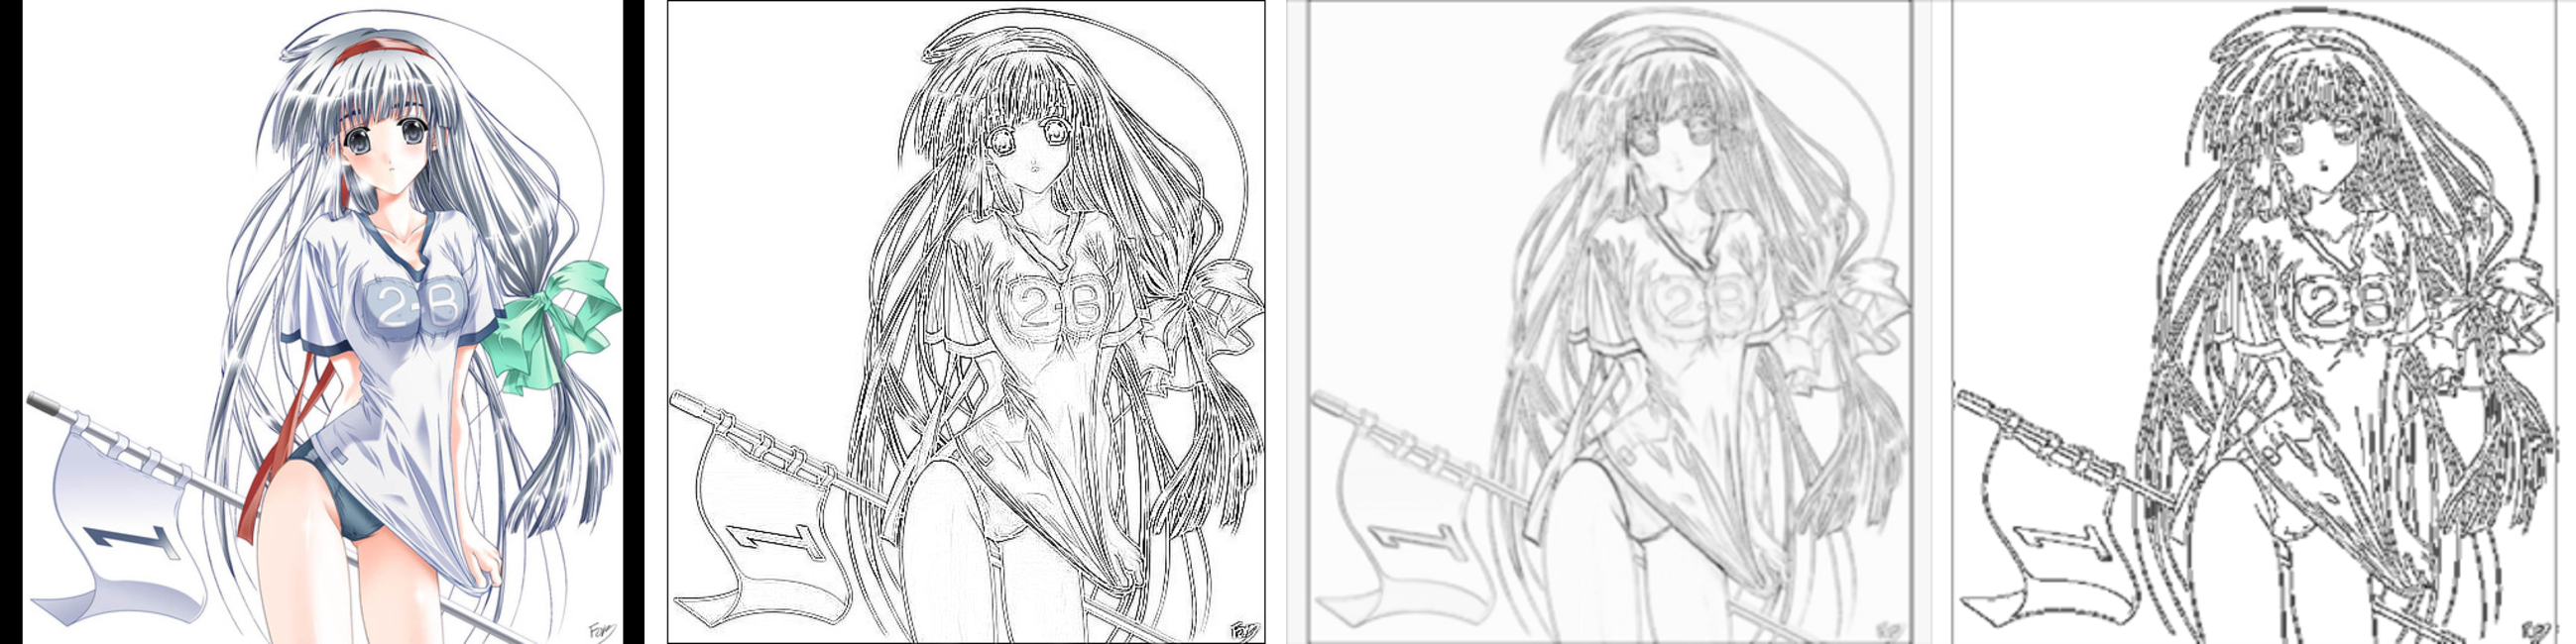
\includegraphics[width=\textwidth]{edge}
	\caption{각각의 edge detection 알고리즘 결과 비교. 가장 왼쪽 그림은 원본 이미지이고, 왼쪽에서 두 번째 그림이 PIL의 결과이다. 왼쪽에서 세 번 그림은 HED, 오른쪽 그림은 Canny Detection 알고리즘의 결과이다}
	\label{fig:edge_detection}
\end{figure}
각각의 결과를 확인한 뒤, 내부 의견 조율로 우리는 PIL의 edge detection 알고리즘을 사용하기로 결정하였다. 

그러나 이 방법만 적용하기에는 스케치라기엔 거친 느낌이 강해서, 이를 완화할 수 있는 추가적인 처리 과정을 강구하였다.
이를 위해 적용한 방법은 두 가지이다.
첫 번째는 Edgar Simo-Serra 외 3명이 제안한 딥러닝 기반의 Sketch Simplification 기술이고 \cite{SimoSerraTOG2018}, 두 번째는 PIL의 자체 이미지 smoothing 필터를 적용하였다 (그림 \ref{fig:edge_smooth}).
하지만 Sketch Simplification은 전체적으로 스케치 이미지를 불분명하게 만드는 효과가 있었고, smoothing 필터를 적용한 이미지는, 초기의 거친 느낌을 잡아주었기 때문에, 최종적으로는 PIL edge detection - PIL Smoothing Filter를 순차적으로 적용하여 sketch 이미지를 만드는 것으로 사용하기로 결정했다.
\begin{figure}[t]
	\centering
	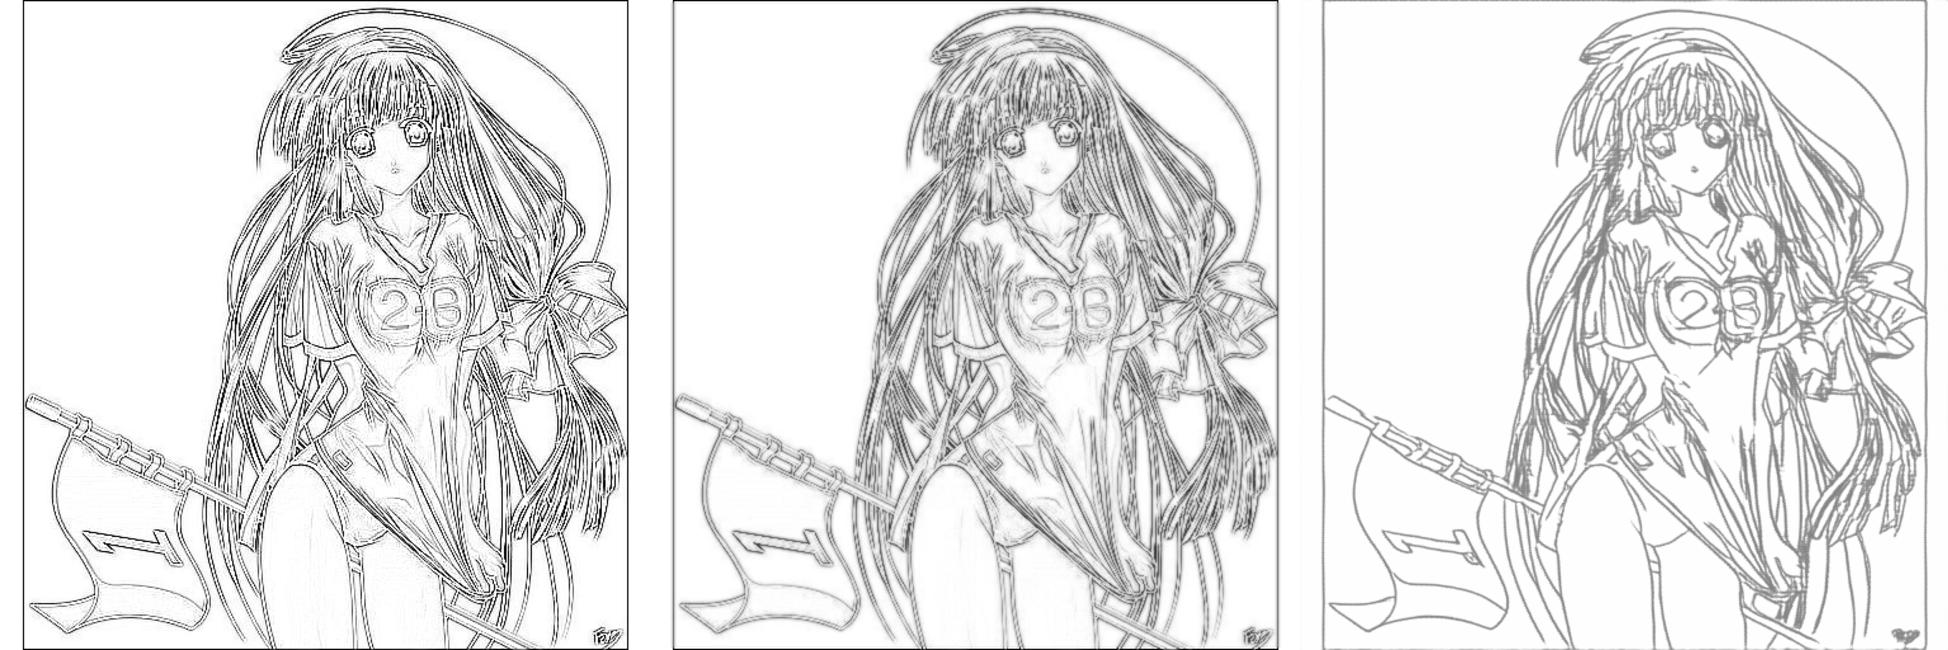
\includegraphics[width=\textwidth]{smooth}
	\caption{PIL edge detection을 통해 얻은 스케치 이미지에 적용한 추가적인 효과. 가장 왼쪽이 edge detection을 통해 뽑아낸 직후이고 (그림 \ref{fig:edge_detection}의 왼쪽에서 두 번째 그림과 동일), 가운데가 이 그림에 Sketch Simplification을 적용한 그림, 가장 오른쪽이 smoothing filter를 적용한 그림이다. 그림에서 확인할 수 있듯이, Sketch Simplification을 적용하면 머리카락 같이 세세하고 많은 스케치를 제대로 잡아내지 못한다.}
	\label{fig:edge_smooth}
\end{figure}

\subsubsection{Image Resizing/Scaling}

Danbooru 2017 데이터셋은 모든 이미지가 우리가 정한 512 x 512 픽셀 사이즈이지만, Niko 데이터셋은 이미지 별로 사이즈가 천차만별이다.
따라서 우리는 이에대해 학습 및 추론시, 추가적인 resize작업과, scaling 작업이 진행될 수 있도록 하였다.
Resize 작업에 대해서는, 주어진 이미지 파일의 가로 (세로) 길이 중 512 픽셀이 안 되는 쪽이 있다면 그 방향에 대해서는 양 옆으로 흰 색으로 패딩해주었다.
그 후 이미지의 중심을 기준으로 512 x 512 크기로 잘라서, 딥러닝 모델에 input으로 들어갈 수 있도록 하였다 (Center Crop).

이미지 scaling은 Phillip Isola \cite{phillip2017}등 다른 일반적인 image translation 문제에서 사용하는 방법을 사용하였다. 하나의 RGB 픽셀 값이 가질 수 있는 값은 $[0, 255]$ 사이의 정수 값이므로 원래의 픽셀 값은 $p$, scale된 픽셀 값을 $\hat{p}$라고 하자. Generator 모델에서 마지막 레이어의 feature가 tanh 비선형 활성함수를 통과하기 때문에
\begin{align}
	\hat{p} = (2 \times \frac{p}{255.0}) - 1 && \text{where $p \in [0, 255]$ integer value}
\end{align}
이와 같이 scale될 수 있도록 하였다. 이렇게 하면 $\hat{p} \in [-1, 1]$을 만족하는 실수 값이 되고, 이는 실제 이미지와 만들어진 가짜 이미지가 가질 수 있는 픽셀 값의 범위를 같게 만들게 된다.

\subsection{Style2Paint Reproduction}

앞서 기술하였지만, 일반적인 딥러닝 논문들과 달리, \stylepaint 는 코드 공개 없이 논문에 아이디어만 제시하여두고, 구체적인 모델 구조나, 학습 파라미터 설정 값들은 대체로 기재하지 않았다.
또한 담당자님의 말에 의하면, 논문에 나온 내용도, 틀린 부분이 많아서, 저대로 실험하면 결과가 안 나올 것이라는 얘기를 들었다. 
이에 따라, 우리는 이 논문의 모델을 결과를 최대한 재생산 하는 것이 앞으로의 원활한 프로젝트 진행에 있어서 중요할 것이라고 판단을 하였고, 중간평가까지의 목표로 삼았다.